\documentclass[a4paper]{report}
\usepackage[justification=centering]{caption}
\usepackage{fancyhdr}
\usepackage{float}
\usepackage[top=2.54cm, bottom=2.54cm, left=1.91cm, right=1.91cm]{geometry}
\usepackage{graphicx}
\usepackage[utf8]{inputenc}
\usepackage{subfig}
\usepackage{amsmath}
\usepackage{multicol}
\usepackage{bm}
\usepackage{amsfonts}


\setlength{\parindent}{0pt}
\renewcommand*\thesection{\arabic{section}}

\begin{document}
\thispagestyle{fancy}
\lhead{Quentin Walger\newline Micka\"el Vincenti}
\chead{Model Predictive Control - Quadcopter}
\rhead{\today}

\section*{Getting acquainted - nonlinear model and linearization}

Since the state-space representation is $\dot{\bm{x}} = A_c \bm{x} + B_c \bm{u}$, and the vectors $\bm{x}, \bm{u}$ have the following dimensions: $\bm{x} \in \mathbb{R}^{12}$ and $\bm{u} \in \mathbb{R}^{4}$, it is normal that $A_c \in \mathbb{R}^{12 \times 12}$ and $B_c \in \mathbb{R}^{12 \times 4}$.

\subsection*{1. Interpretation of structure of matrices $A_c$ and $B_c$}

We have the following state-space representation: \\

Regarding the matrix $A_c$, the lines $1$ to $3$ are stating $[\dot{x}, \dot{y}, \dot{z}] = [\dot{x}, \dot{y}, \dot{z}]$. It is the same for the derivatives of the variables $\alpha, \beta$ and $\gamma$ in the lines $7$ to $9$. \par
The lines $4$ and $5$ are stating $\ddot{x} = g \cdot \beta$ and $\ddot{y} = -g \alpha$, with $g$ the gravitational constant -- > $\bm{WHY}$. \\

Regarding the matrix $B_c$: \par
- Line $6$: We have $\ddot{z} = 3.5 \cdot \sum_{i = 1}^4 u_i$: \par
The acceleration of the non-rotational origin $\ddot{\bm{O}}_B$ is only present in the $z$ coordinate and is $\ddot{z}_s = -g + \frac{F}{m}$, with $F = k_f \cdot [\sum_{i = 1}^{4} u_i]$. By taking the value of $k_f$ in the first row of \texttt{quad.K} and the value of $m$ in \texttt{quad.mass}, this leads to $\frac{k_f}{m} = \frac{28}{8} = 3.5$. \\

- Lines $10$ to $12$: $\begin{bmatrix} \ddot{\alpha} \\ \ddot{\beta} \\ \ddot{\gamma} \end{bmatrix} = \begin{bmatrix} 0 & 0.56 & 0 & -0.56 \\ -0.56 & 0 & 0.56 & 0 \\ 0.73 & -0.73 & 0.73 & -0.73 \end{bmatrix} \bm{u}$:\par
We know that $\omega_s = \begin{bmatrix} \dot{\alpha_s} \\ \dot{\beta_s} \\ \dot{\gamma_s} \end{bmatrix} = \begin{bmatrix} 0 \\ 0 \\ 0 \end{bmatrix}$. We also know that \par 
$\dot{\omega}_s |_{\omega_s = \bm{0}} = \begin{bmatrix} \ddot{\alpha} \\ \ddot{\beta} \\ \ddot{\gamma} \end{bmatrix} \Big |_{\omega_s = \bm{0}} = \mathcal{I}^{-1} \begin{bmatrix} M_\alpha \\ M_\beta \\ M_\gamma \end{bmatrix} = \mathcal{I}^{-1} \begin{bmatrix} 0 & k_F L & 0 & - k_F L \\ -k_F L & 0 & k_F L & 0 \\ k_M & -k_M & k_M & -k_M \end{bmatrix} \bm{u}$. \par
The matrix \texttt{quad.L} gives $L = 0.2$ and \texttt{quad.km} gives $k_m = 11$. Since \texttt{quad.I} = $diag(10, 15, 15)$ and $k_F = 28$, we have $\mathcal{I}^{-1} = diag(0.1, 0.1, \frac{1}{15})$. This leads to $\begin{bmatrix} \ddot{\alpha} \\ \ddot{\beta} \\ \ddot{\gamma} \end{bmatrix} = \begin{bmatrix} 0 & 0.56 & 0 & -0.56 \\ -0.56 & 0 & 0.56 & 0 \\ 0.73 & -0.73 & 0.73 & -0.73 \end{bmatrix} \bm{u} $.

\section*{First MPC Controller}
\subsubsection*{1. Choice of tuning parameters and motivation for them}

First, the matrices $Q$ and $R$ are set to identity matrices. Those parameters give the results in Fig. \ref{Q1}. We see that the roll and pitch angles take far too much time too reach steady-state. Thus, the states $\alpha$ and $\beta$ have to be more penalized, namely the state penalty matrix is set to $Q = \text{diag}(1,\ 100,\ 100,\ 1,\ 1,\ 1,\ 1)$. The results are shown on Fig. \ref{Q100}.

\subsubsection*{2. Plots of the response to an appropriate initial condition}

\begin{figure}[H]
	\centering
	\subfloat[]{\fbox{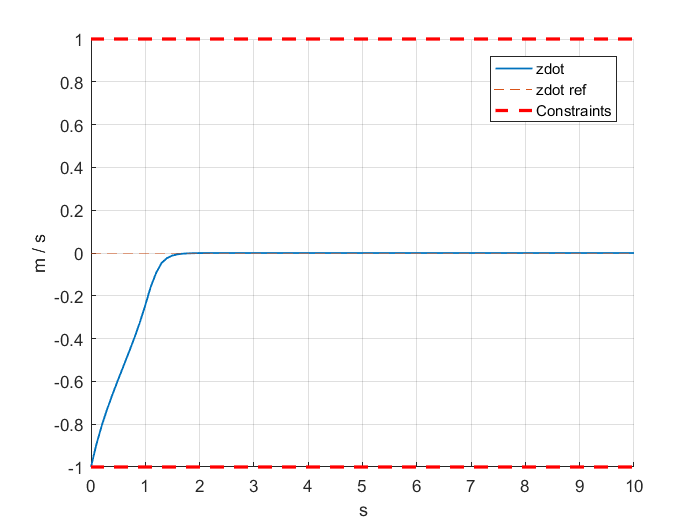
\includegraphics[scale=0.25]{z_rate_Q1.png}}}
	\quad
	\subfloat[]{\fbox{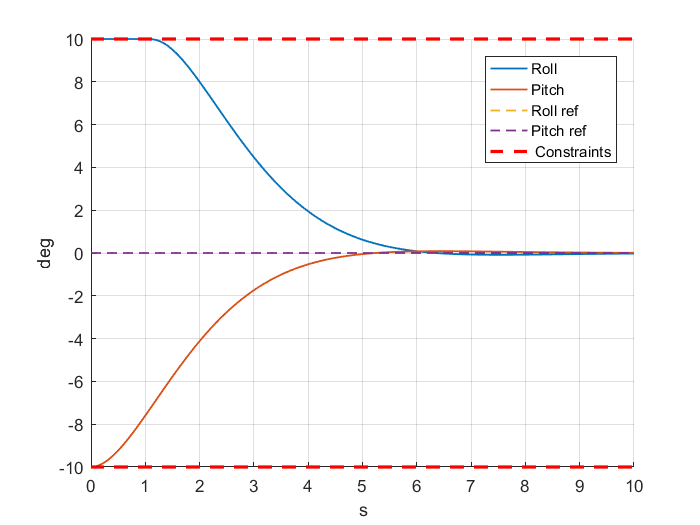
\includegraphics[scale=0.25]{roll_Q1.png}}}
	\quad
	\subfloat[]{\fbox{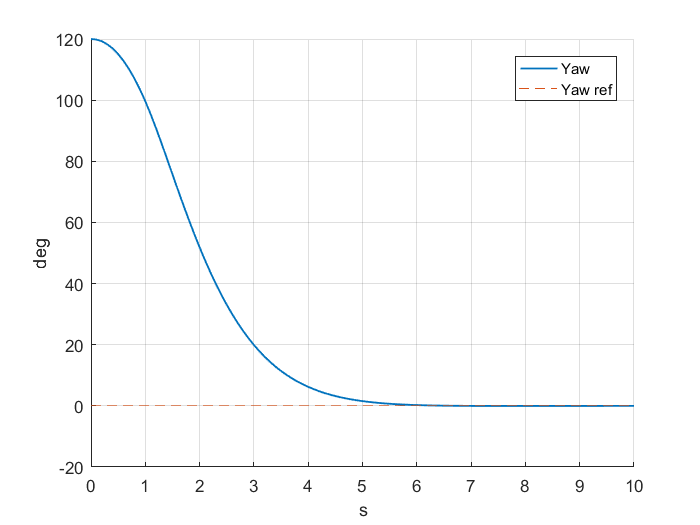
\includegraphics[scale=0.25]{yaw_Q1.png}}}
	\quad
	\subfloat[]{\fbox{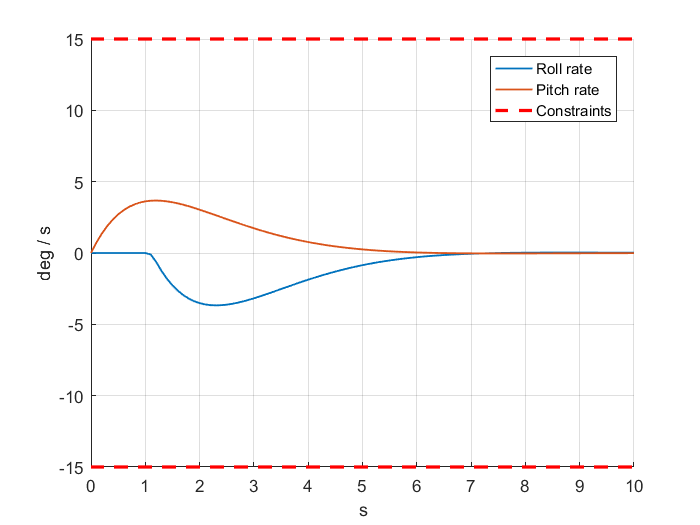
\includegraphics[scale=0.25]{roll_rate_Q1.png}}}
	\quad
	\subfloat[]{\fbox{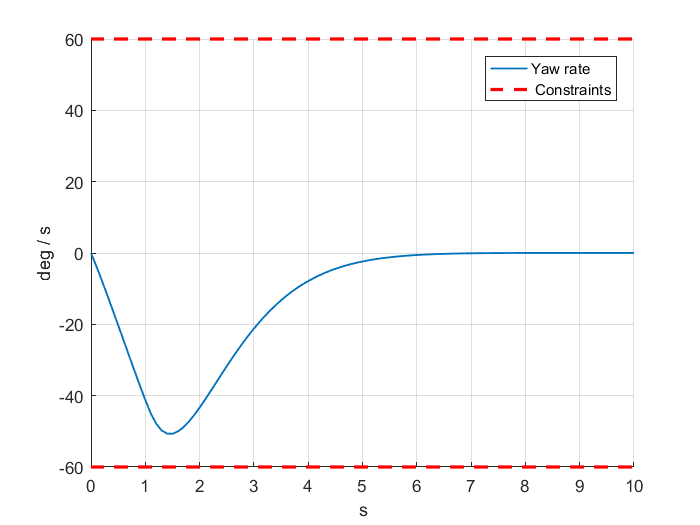
\includegraphics[scale=0.25]{yaw_rate_Q1.png}}}
	\quad
	\subfloat[]{\fbox{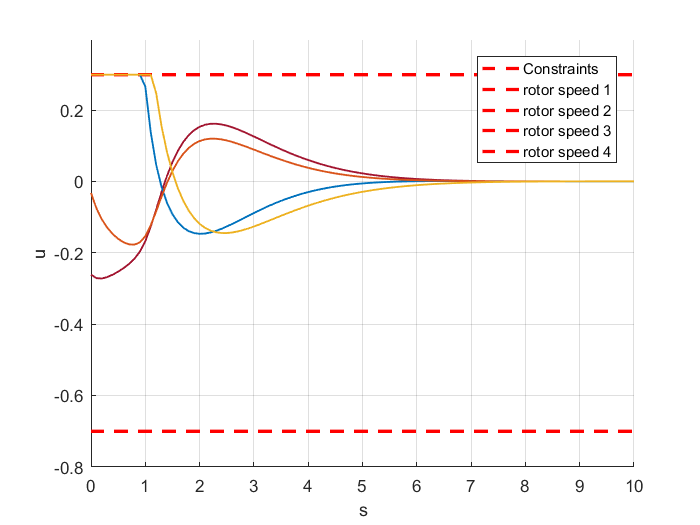
\includegraphics[scale=0.25]{rotor_speed_Q1.png}}}
	\caption{\small{(a) $\dot{z}$, (b) $\alpha,\ \beta$, (c) $\gamma$, (d) $\dot{\alpha},\ \dot{\beta}$, (e) $\dot{\gamma}$, (f) $u$}}
	\label{Q1}
\end{figure}

\begin{figure}[H]
	\centering
	\subfloat[]{\fbox{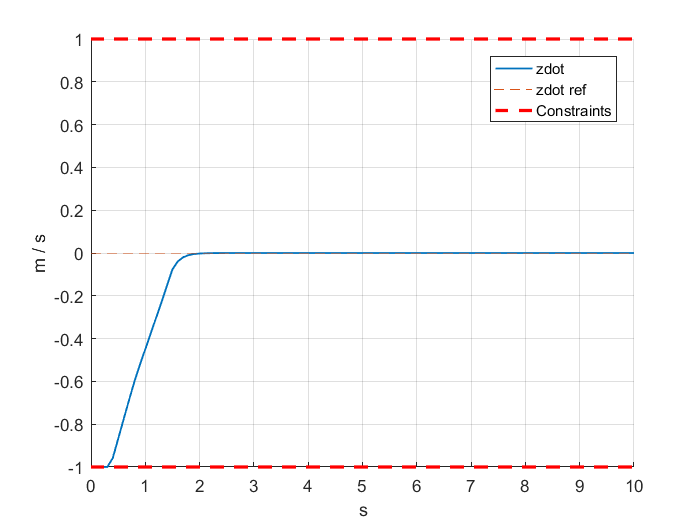
\includegraphics[scale=0.25]{z_rate_Q100.png}}}
	\quad
	\subfloat[]{\fbox{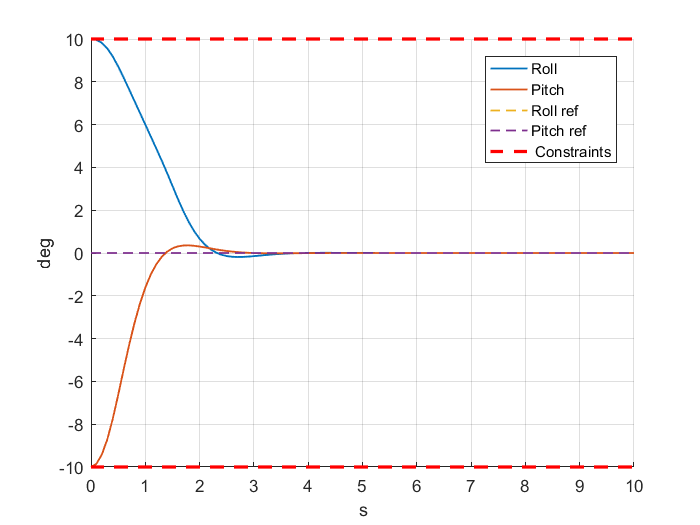
\includegraphics[scale=0.25]{roll_Q100.png}}}
	\quad
	\subfloat[]{\fbox{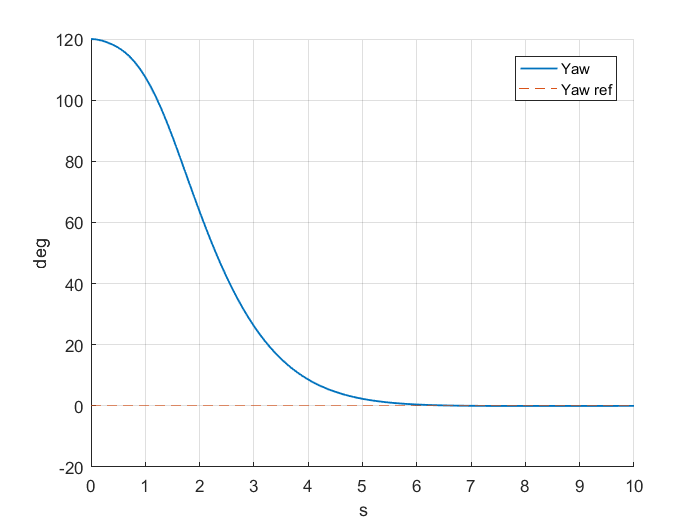
\includegraphics[scale=0.25]{yaw_Q100.png}}}
	\quad
	\subfloat[]{\fbox{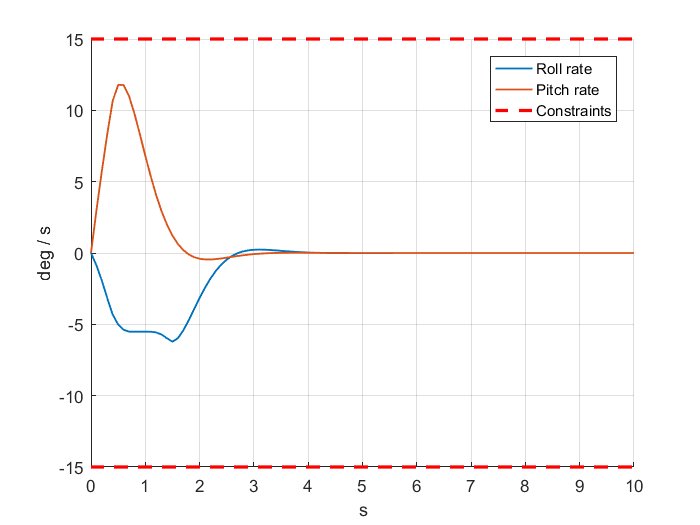
\includegraphics[scale=0.25]{roll_rate_Q100.png}}}
	\quad
	\subfloat[]{\fbox{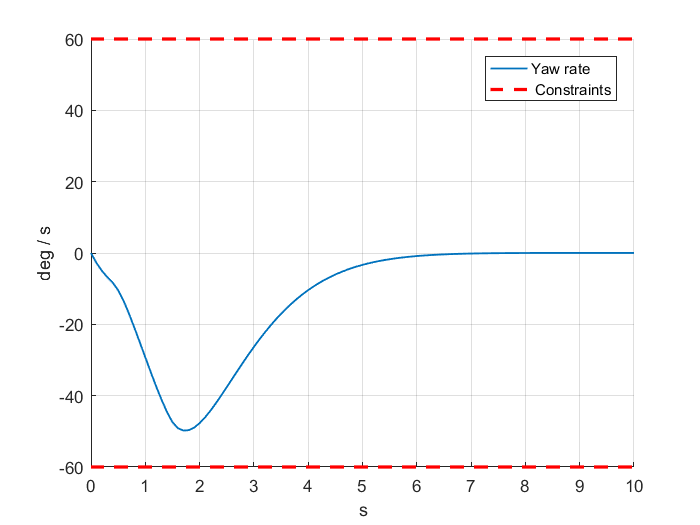
\includegraphics[scale=0.25]{yaw_rate_Q100.png}}}
	\quad
	\subfloat[]{\fbox{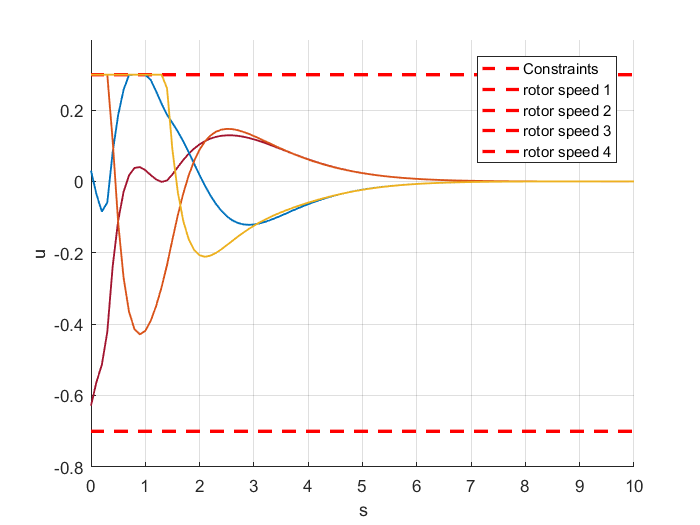
\includegraphics[scale=0.25]{rotor_speed_Q100.png}}}
	\caption{\small{(a) $\dot{z}$, (b) $\alpha,\ \beta$, (c) $\gamma$, (d) $\dot{\alpha},\ \dot{\beta}$, (e) $\dot{\gamma}$, (f) $u$}}
	\label{Q100}
\end{figure}


\section*{Reference tracking}
\subsection*{Deliverables}
\subsubsection*{Interpretation of the solution $(\bold{x}_r; \bold{u_r})$ to system (4) for arbitrary $\bold{r}_1$}
\subsubsection*{plots of the response to a constant reference signal}
\subsubsection*{plots of the response to a slowly varying reference signal}

\section*{First simulation of the nonlinear model}
\subsection*{Deliverables}
\subsubsection*{plots of a reference tracking response of the nonlinear model}

\section*{Offset free MPC}
\subsection*{Deliverables}
\subsubsection*{motivation for the choice of the estimation error dynamics}
First, we need to be sure that the system is observable. This is done by verifying that, in the initial system: \par
$ \left\{
      \begin{aligned}
        \,x^+& =& A_1\,x& + B\,u +& B_d\,\bar{d}&\\
        \,\bar{d}^+& =& & & \bar{d}& \\
        \,y& =& C\,x& +& C_d\,\bar{d}& \\
      \end{aligned}
    \right.
$ \par
We can identify the matrices $B_d, C = diag(\bold{1}_7)$ and $C_d = diag(\bold{0}_7)$, with $\bold{1}_n$ is a vector of ones $\in \mathbb{R}^n$ (same for $\bold{0}$), and $diag(vec)$ is a matrix with the elements of $vec$ in the diagonal $\in \mathbb{R}^{|vec| \times |vec|}$. \\

We have that the rank of the matrix $\begin{bmatrix} C \\ CA_1 \\ \vdots  \\ CA_1^{N-1} \end{bmatrix}$ is $n_x = 7$ and the rank of the matrix $\begin{bmatrix} A_1 - I_7 & I_7 \\ C & C_d \end{bmatrix}$ is $n_x + n_d = 14$. \par
The two conditions are verified using the "rank" command on Matlab. \\

We are choosing a dead-beat observer: this observer is taking the observability error to $0$ in $n = n_x + n_d$ samples, which corresponds to $n \cdot T_s = 14 \cdot 0.1 = 1.4s$. \par


\subsubsection*{step reference tracking plots in the presence of disturbance}
\subsubsection*{slowly-varying reference tracking plots in the presence of disturbance}



\end{document}